\documentclass[twocolumn]{article}
\linespread{1.0} 
\usepackage{amsmath, amssymb, amscd, amsthm, amsfonts}
\usepackage{graphicx}
\usepackage{hyperref}
\usepackage[top=100pt,bottom=100pt,left=100pt,right=100pt, lineheight=1.5]{geometry}

\title{Questionnaire Research Paper}
\author{Phillip Eismark, Veronique Jensen, Jack Zhong, Martine Magh}
\date{Marts 2020}

\newtheorem{theorem}{Theorem}
\newtheorem{lemma}[theorem]{Lemma}
\newtheorem{conjecture}[theorem]{Conjecture}

\newcommand{\rr}{\mathbb{R}}

\newcommand{\al}{\alpha}
\DeclareMathOperator{\conv}{conv}
\DeclareMathOperator{\aff}{aff}

\begin{document}

\maketitle

\begin{abstract}
This paper documents the findings and analysis on the correlation between the student satisfaction of their course and the instructor's influence on the matter. The paper will answer the projectgroup’s defined research question as well as several sub-questions based on the dataset, which will correspond to be the central part of the paper.  
\end{abstract}

\section{Introduction}\label{section-introduction}

In this assignment, we have been tasked to perform a statistical data analysis by the given dataset and document the process in the form of a report.  
Teaching is the instructor's most valuable tool to achieve educational goals. An Instructor must be able to manage the students and improve their ability by using their competence, attitudes and teaching methods to deliver and teach the material/curriculum.Students' level of satisfaction has a strong effect on their learning success or failure.

This paper is built on the analysis of a data set based on 5820 students' answers to a satisfaction questionnaire.

\section{Research Question}\label{section-topological}

Is there a correlation between the level of the student satisfaction of the course and the instructors assessed by; the rating of the level of respect, openness and competence?
Sub-questions:
How do we define and rate the students' level of satisfaction?
How do we define and rate the attributes that we use to describe the instructors level of respect, openness and competencies?


\section{Methods}\label{section-colored}

In this paper we are basing our research of a questionnaire given to 5820 students. The questionnaire contains information about the class, number of times the class has been taken by the student, attendance and difficulty. After that there are 28 questions all regarding the student’s thoughts of the course and the course instructor. The questions are all of “Likert” - type, which means that the questions are answered with values rating from 1 to 5. We have decided that 1 means that the student strongly disagrees with the question and 5 means that they strongly agree.
All the entries are anonymous in order to ensure that the students give honest answers, therefore we only know the instructor id and class/course id.
 
We are using these empirical findings to try and support our hypothesis that there is a correlation between the competence and openness of an instructor and the student’s satisfaction of the course. The study therefore follows the formulated and vertificational research method mentioned in Nunamaker et al. paper, as we are trying to \emph{“identify problems for more precise investigation, to develop hypotheses, as well as to gain insights and to increase familiarity with the problem area”} 
Furthermore our entire purpose of the research is to gain evidence that either supports or refutes our hypothesis\cite{Nuna}. 
 
In the following analysis we are going to be exploring whether there is a correlation between the student’s satisfaction of the course and the student’s opinion regarding the instructor on two different topics, namely the instructor’s competence and openness. We are also going to be justifying why we have chosen to look at those topics in particular and which questions we think describe exactly those topics.


\section{Analysis}\label{section-intersection}

In this section, we’re covering the analysis of the dataset by finding the correlation between the data inside and explaining our thoughts and hypothesis regarding our choices. 
We have structured a table, which shows the pairing of each question from the given dataset and our defined categories. 
\\
\begin{center}
\begin{tabular}{ |p{3cm}|p{3cm}|p{4cm}|p{4cm}|}
 
\hline
Group/Thing to describe & Questions \\
\hline
The student's level of satisfaction & Q3, Q5, Q9, Q10, Q11, Q12 \\
\hline
The instructor's openness & Q21, Q22, Q23, Q24, Q27, Q28  \\
\hline
The instructor's level of competence & Q13, Q14, Q15, Q16, Q18, Q19, Q20 \\
\hline
\end{tabular}
\end{center}
\\
\subsection{The students level of satisfaction}
To help answer the research questions, we needed to define what exactly a student's level of satisfaction implies. The questions that we grouped into group 1 where all questions that were descriptive of a students satisfaction. 
The major responsibilities of instructors are to deliver an effective service in the form of teaching. For an instructor to educate well, they must have a certain level of competence. Competence is the ability to do something well.
There is a relationship between a student’s satisfaction and a teacher’s competence, preparation and their level of respect for the student. To identify this relationship, we have to analyze the data set and find connections between the different questions. We found that questions 3 and 5-10 tell us about student satisfaction in various ways. The questions revolve around an individual student’s experience with the assigned course and instructor. 

\subsection{The instructors openness}
Before commencing and grouping the different data set questions into the category, we first have to define the meaning behind the word, “Openness”. According to the Macmillan Dictionary, the meaning behind the word is “an honest way of talking or behaving in which you do not try to hide anything” and “a tendency to accept new ideas methods and changes”\cite{Macmillan}. With a better understanding of the word, “Openness”, we could proceed to work with the data set. This category is mainly focused around an instructor's capability of committing to an open environment, where the individual instructor is able to engage a student with their level of openness. An instructor's interaction with a student can have a high influence on the students comfort level around the assigned instructor. What we're looking for is whether the instructor of the course barricades a wall between themselves and the students. But we're also looking into whether the instructor is able to devote themselves into closing the comfortability gap between instructor and student.The reason as to why the questions are listed in the category from the table above, is because they all share common interests. The questions were mainly based around the individual instructor’s work ethic and actions, which therefore correlates with the category. The questions are viable to the category, because they are centered around each instructor, where the answer to these questions involves the students' opinions about the instructors.  

\subsection{The Instructors Level of Competence}
Firstly, to answer whether the instructors level of competence could be correlated to the students level of satisfaction, we needed to define what exactly competence implies. 
Our initial thoughts on a competent instructor would be one with traits, that not only helps him communicate abstract ideas in a digestible way, but also clearly understands what the student needs to hear to come to a realisation. The Oxford dictionary defines competence as doing something successfully or efficiently “The ability to do something successfully or efficiently”\cite{Oxford} and Wikipedia defines competence like this: “Competence is the set of demonstrable characteristics and skills that enable, and improve the efficiency of, performance of a job”\cite{Wiki}. We decided to go with these definitions as we thought that this matched our initial thoughts as well as the data set. After defining the meaning of competence we were able to look at the data set and group the questions that support this definition. The requirements for a question to be accepted in to the group, called “group 3”. Was that the question would have to cover some aspect of our definition of competence. For example, question 19: “The Instructor made effective use of class hours” are describing the efficiency of the instructor and thereby also describing some aspect of the level of competence. Whereas question 17: “The Instructor arrived on time for classes” were omitted, because it does not describe the instructors competence, e.g the instructor is not worse at communicating and formulating ideas because he is late. Though, it can be argued that an instructor being late could worsen the performance and efficiency at which the instructor is performing, but because it is unclear why the teacher is late, and that this is also a matter of what the individual student thinks is acceptable, we chose to not add it to the competence group. After defining our groups we were able to run a pandas profiling to help us achieve a fast overview of the data. We created three data sets, openness, satisfaction and competence which each of them consisted of the questions we have grouped. From here we were able to apply Pearson’s r on the data.


\section{Findings}\label{section-universal}
\subsection{Pearson's R}
By using “Pearson’s correlation measurement”\cite{Pearson}, also referred to as “Pearson’s r”, we could identify the strong correlations between the groups that we categorized and the students' level of satisfaction. 
\\
\begin{figure}
\centering
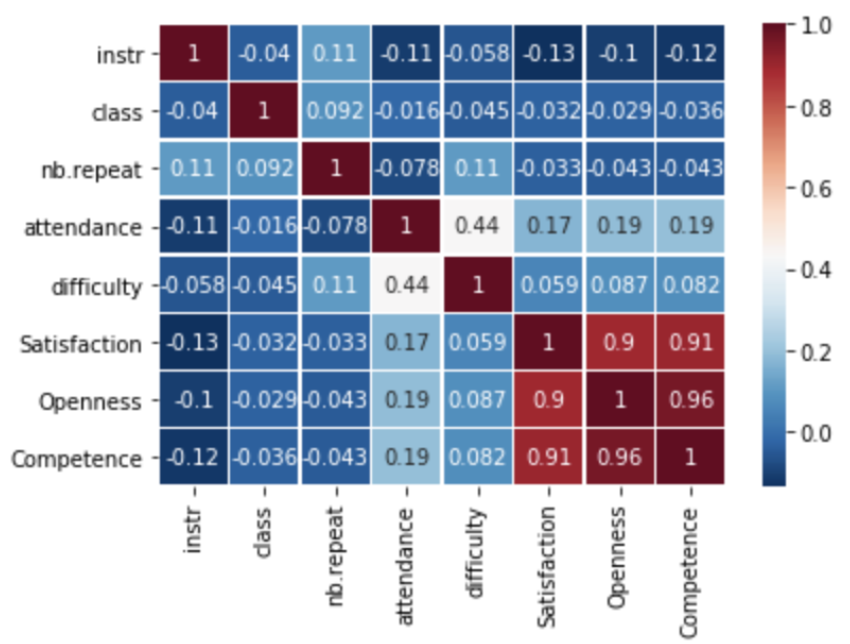
\includegraphics[width=7cm]{Figures/pictures/pearson.png}
\caption{Pearson's R}
\label{fig:pearson}
\end{figure}
\\
As the heatmap in figure 1 shows, there is a correlation of 0,91 between the two groups Competence and Satisfaction. This means that these two groups are highly correlated. The model also shows that there is a strong correlation of 0.96 between the student’s satisfaction of the course and the instructor’s openness.

\subsection{Average ranking of the instructors}
During our analysis of the data it also became apparent that there was a big difference in the number of students, and therefore classes, the three instructors had. We wondered if there could be a correlation between an instructor with a lot of classes, who therefore had more to do and prepare, and his/her students’ rating of the course.


In the two diagrams in figure 2 we can see that the instructor with the most students and classes, instructor 3, is also the instructor who has gotten the lowest rating concerning satisfaction, openness and competence. 
So this could point to the fact that instructors with many classes have less time for preparation, and therefore the overall evaluation of that class isn’t as good as it would be if the instructor had more time.
\begin{figure}
\centering
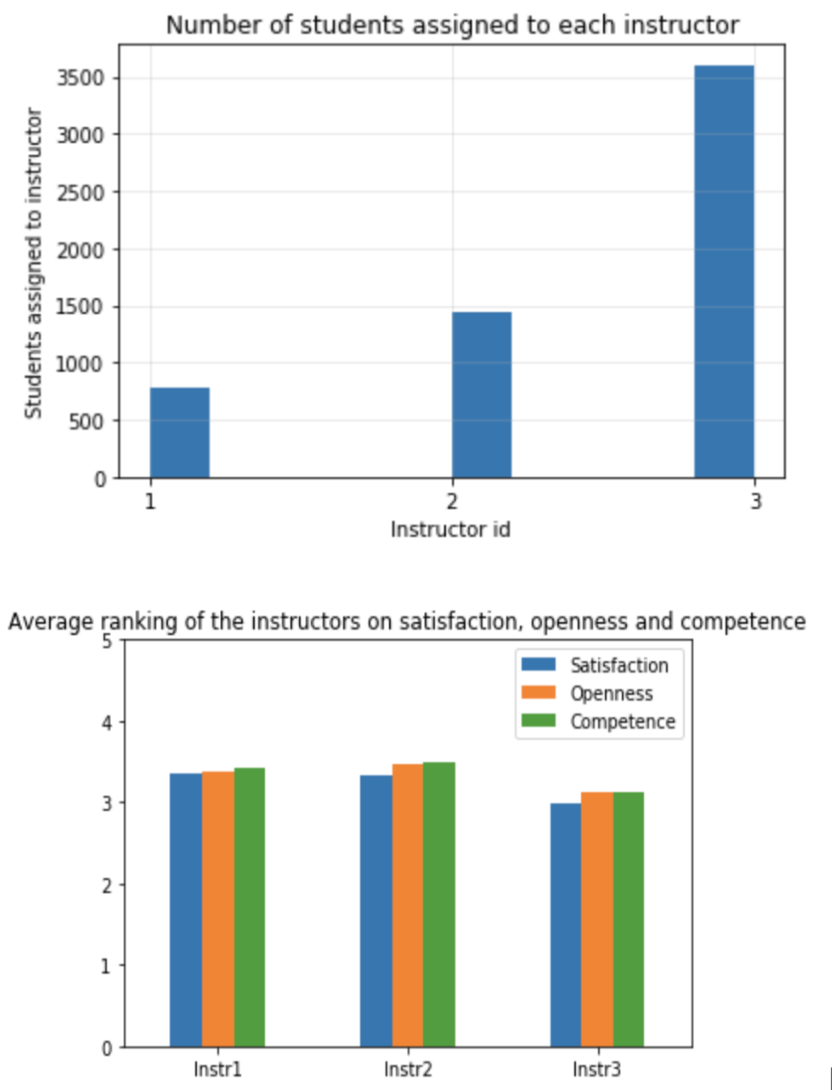
\includegraphics[width=7cm]{Figures/pictures/billede2.png}
\caption{The figure on the left shows the number of students assigned to each teacher. The figure on the right shows the average rating of the instructor}
\label{fig:pearson}
\end{figure}


\section{Conclusions}\label{section-applications}
This paper set out to answer the research question that asked if there was a correlation between the satisfaction of a student and the teachers competence and openness. The research and findings are based on a questionnaire, which means that we would have to analyse the data and model it in a way that was useful to answer our research question. This means we used empirical findings to try and answer our research question, with the formulated and vertificational research method. The findings show us through a Pearon’s r model that the hypothesis we had, that there is a correlation between the teachers competence and openness, with the level satisfaction that the student has towards the course.

\section{Notebook}\label{section-applications}
Link to GitHub: 

\begin{thebibliography}{9}

\bibitem{Oxford} The Oxford Dictionary
\\\textit{The Oxford Dictionary}.  \\\textit{https://www.lexico.com/en/definition/competence}

\bibitem{Wiki} Wikipedia
\\\textit{Wikipedia}.
\\\textit{https://en.wikipedia.org/wiki/Competence_(human_resources)}

\bibitem{Nuna} Nunamaker et al 1990
\\\textit{Systems Development in Information Systems Research.}
\\\textit{Course material}

\bibitem{Macmillan} Macmillan Dictionary
\\\textit{Openness definition}
\\\textit

\bibitem{Pearson} Pearson r
\\\textit{Pearson correlation coefficient}
\\\textit{https://en.wikipedia.org/wiki/Pearson_correlation_coefficient}

\end{thebibliography}

\end{document}
